Was war geschehen? Nachdem 1945 \ac{vuz} der Faschismus besiegt und der Zweite
Weltkrieg beendet war, konnte die im Krieg notgedrungen herrschende
keynesianistische Wirtschaftspolitik ausgeweitet werden, was zu einem Boom in 
den westlichen Staaten führte, der bis in die 1960er Jahre \ac{vuz} anhielt --
die >>Goldene Zeit<< des Kapitalismus.
In den 1970er Jahren \ac{vuz} geriet die Weltwirtschaft allerdings in eine neue
Krise: Deregulierung, Entschlackung des Staates, Steuersenkungen, Outsourcing,
Globalisierung und Finanzkapitalismus waren die Folge. 
Die unter dem schwammigen Begriff des \emph{Neoliberalismus} zusammengefassten
Entwicklungen kündigten die scheinbare Rettung des globalen
Kapitalismus an.
Doch auch diese >>Rettung<< war von nur kurzer Dauer. 
2008 \ac{vuz} brach der Finanzmarkt zusammen und für fast zwei Jahrzehnte
befanden sich die meisten (westlichen) Staaten in einer andauernden
Akkumulationskrise, die von dem Aufstieg der ehemaligen Schwellenländer
(insbesondere China und Indien) noch verschärft wurde. 
Nach einer globalen Pandemie und dem Ausbruch des \emph{East-European-Conflict},
in dem erstmals seit dem Zweiten Weltkrieg Nato-Truppen auf Russische Soldaten
trafen, stand die Weltwirtschaft erneut kurz vor dem absoluten Zusammenbruch. 
Während sich die aufstrebenden Schwellenländer und Industriestaaten des
globalen Südens noch halten konnten, standen speziell die westlichen Staaten
kurz vor dem wirtschaftlichen Totalkollaps. 
Allen voran die USA beantworteten die Krise mit protektionistischen Maßnahmen
und einem Schulterschluss der Techgiganten mit der republikanischen US-Politik.
Während die Entwicklung in Europa sich zunächst der amerikanisch Politik
anzuschließen schien, kam es kurz vor dem Ausbruch eines globalen Krieges im
Jahre 2026 \ac{vuz} zu einem überraschenden Wahlsieg der Sozialdemokratie in
mehreren großen Wirtschaftsnationen Westeuropas: England, Frankreich, Italien,
Griechenland, Deutschland, Spanien, Polen.
Einige Utopisten wagten leise zu hoffen, dass sich endlich unter der Führung
Europas die Länder der Welt entscheiden würden, Rosa Luxemburgs Losung --
Sozialismus oder Barbarei -- in Richtung einer weltweiten Roten-Umwälzung
aufzulösen, doch weit gefehlt!
Zwar konnte das geschlossene Auftreten des sozialdemokratischen Europas einen
Beginn des Krieges aufhalten, doch nur indem sie auf globaler Ebene
weitreichende Strukturreformen durchsetzten, die -- wie schon zu Beginn der
2000er Jahre \ac{vuz} -- die Interessen des Kapitals bedienten, um in der
verschärften Konkurrenz überlebensfähig zu bleiben.
Erneut rettete die Sozialdemokratie also die kapitalistische Weltordnung auf 
Kosten derjenigen, die sie eigentlich vertreten sollte\dots

\section{Strukturreformen} 
Um den Frieden zu sichern und die Welt vor einem drohenden Totalkollaps zu
retten, konnten weitreichende Strukturreformen durchgesetzt werden, die
Geopolitik, Wirtschaft, Kultur und zahlreiche andere Bereiche betraf. 

\subsection{Aufteilung der Welt} 
Der wohl zentralste und folgenreichste geopolitische Aspekt war die Aufteilung
der Welt in zwei fixe Blöcke: der blaue Block (unter Führung der USA) und der
rote Block (unter Führung Chinas). Nur sehr wenige Länder blieben neutral.\\\\
%
\textbf{Wichtigste Länder des blauen Blocks:}\\
\emph{USA, Deutschland, Japan, Vereinigtes Königreich, Frankreich, Kanada, Südkorea,
Italien, Türkei, Iran.}\\
\textbf{Wichtigste Länder des roten Blocks:}\\
\emph{China, Russland, Brasilien, Indonesien, Mexiko, Südafrika, Saudi-Arabien,
Argentinien, Pakistan.}\\
\textbf{Neurale Länder:}\\ 
Schweiz, Nepal, Schweden, Finnland, Mongolei, Singapur, Neuseeland

\begin{center}
  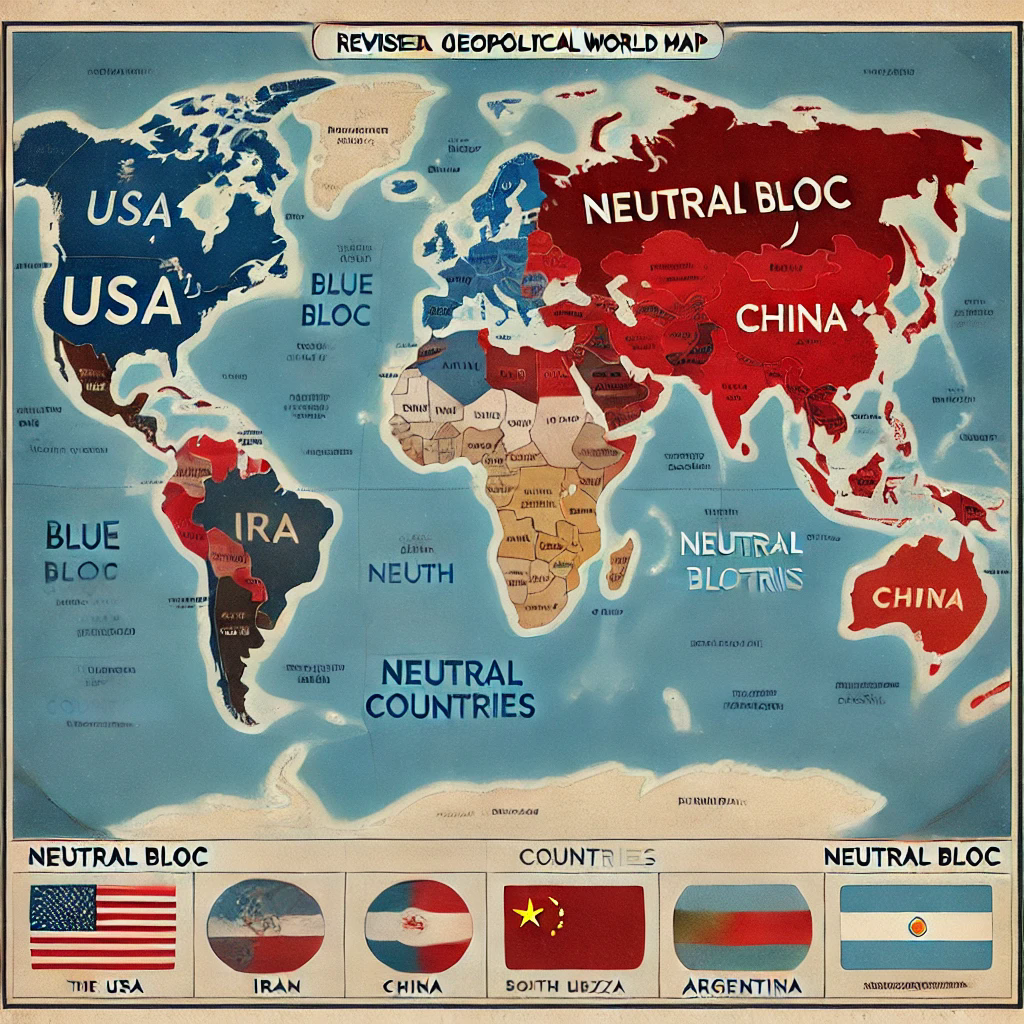
\includegraphics[scale=0.3]{new-world-map.png}%
\end{center}


\subsection{Klassifizierung}
Die wichtigste wirtschaftspolitische Reform war diejenige nach 0.0-, 1.A-, 1.B-
und 5.0-Ländern.
Diese Klassifizierung steht im direkten Zusammenhang mit der neuen Aufteilung
der Welt. 
Während nur die 0.0-Ländern Mandate in der Block-Politik erhielten, stand den
1.A/B-Ländern die Blockwahl frei. Während 1.A Ländern eigenständige
Wirtschafts- und Kulturpolitik freistand, durften 1.B Ländern nur Kulturpolitik
selbstständig entscheiden. 5.0-Länder sollten von nun an unter kompletter
Kontrolle der 0.0-Länder stehen und wurden jeweils einem der Blöcke
zugeordnet.\\\\
% 
Dieser Entdemokratisierung standen allerdings weitreichende wirtschaftliche
Unterstützung entgegen. Während die 0.0-Länder die komplette Wirtschafts- und
Sozialpolitik der meisten anderen Ländern diktieren konnten, waren sie zugleich
verpflichtet 5\% ihres \ac{nil} in 1.A/B-Länder und 7\% ihres \ac{nil} in
5.0-Länder zu investieren. 

\begin{center}
{\def\arraystretch{1.2}\tabcolsep=5pt
  \begin{tabular}{ l || c | c | c | c | l}
    Klassifizierung & BM & W- \& SP & KP & BZ & Invesittionen \\ 
    \hline 
    \hline 
    0.0-Länder & \ch   & \ch & \ch & \cx & {\footnotesize 5\% \ac{nil} -> 1.A/B; 7\% \ac{nil} -> 5.0} \\
    \hline 
    1.A-Länder & (\ch) & \ch & \ch & \cx & {\footnotesize 5\% \ac{nil} -> 5.0} \\
    \hline 
    1.B-Länder & \cx   & \cx & \ch & \cx & {\footnotesize 3\% \ac{nil} -> 5.0} \\
    \hline 
    5.0-Länder & \cx   & \cx & \cx & \ch & \cx \\
    \hline 
    \hline 
    \multicolumn{6}{l}{{\footnotesize \vspace{-0.3cm}\textbf{Legende:} BM =
    Blockmandat, W-\& SP = Wirtschafts- \& Sozialpolitik}}\\
    \multicolumn{6}{l}{{\footnotesize KP = Kulturpolitik; BZ = Blockzwang}}\\
  \end{tabular}
}
\end{center}

\subsection{Neue Zählweise} 
Seit 

\section{Ausbruch des dritten Weltkriegs}


